%**************************************************************************************
% License:
% CC BY-NC-SA 4.0 (http://creativecommons.org/licenses/by-nc-sa/4.0/)
%**************************************************************************************

\documentclass[notes]{beamer}

\mode<presentation> {

\usetheme{Madrid}

% Burnt orange
\definecolor{burntorange}{rgb}{0.8, 0.33, 0.0}
\colorlet{beamer@blendedblue}{burntorange}
% Pale yellow
\definecolor{paleyellow}{rgb}{1.0, 1.0, 0.953}
\setbeamercolor{background canvas}{bg=paleyellow}
% Secondary and tertiary palett
\setbeamercolor*{palette secondary}{use=structure,fg=white,bg=burntorange!80!black}
\setbeamercolor*{palette tertiary}{use=structure,fg=white,bg=burntorange!60!black}

% To remove the footer line in all slides uncomment this line
%\setbeamertemplate{footline}
% To replace the footer line in all slides with a simple slide count uncomment this line
%\setbeamertemplate{footline}[page number]

% To remove the navigation symbols from the bottom of all slides uncomment this line
%\setbeamertemplate{navigation symbols}{}
}

\usepackage{amsmath}
\usepackage{bm}
\usepackage{breqn}
\usepackage{fontawesome}
\usepackage{graphicx} % for figures
\usepackage{subcaption} % for subplots 
\usepackage[labelsep=space,tableposition=top]{caption}
\renewcommand{\figurename}{Fig.} 
\usepackage{cleveref}
\usepackage{caption,subcaption}% http://ctan.org/pkg/{caption,subcaption}
\usepackage{booktabs} % Allows the use of \toprule, \midrule and \bottomrule in tables
\usepackage{multirow}
\usepackage{xcolor}
\usepackage{empheq}
\usepackage[most]{tcolorbox}
\usepackage{listings}% http://ctan.org/pkg/listings
\lstset{basicstyle=\ttfamily,breaklines=true}
\usepackage{siunitx}
\usepackage{verbatim}

% To print 2 slides on a page
%\usepackage{handoutWithNotes}
%\pgfpagesuselayout{2 on 1}[border shrink=2mm]
%----------------------------------------------------------------------------------------
%	TITLE PAGE
%----------------------------------------------------------------------------------------
% The short title appears at the bottom of every slide, the full title is only on the title page
\title[CE 311K: Taylor series]{CE 311K: Taylor series} 
\author{Krishna Kumar} % name
\institute[UT Austin] % institution 
{
University of Texas at Austin \\
\medskip
\href{mailto:krishnak@utexas.edu}{krishnak@utexas.edu} % email address
}
\date{\today} % Date, can be changed to a custom date

\begin{document}

\begin{frame}
\titlepage % title page as the first slide
\end{frame}

\newif\ifshowtoc
\showtoctrue% toggles to show the toc

\AtBeginSection{%
	\ifshowtoc
	\begin{frame}
		\tableofcontents[currentsection, subsectionstyle=show/show/hide]
	\end{frame}
	\fi
}

%----------------------------------------------------------------------------------------
% slides
%----------------------------------------------------------------------------------------
%------------------------------------------------

\section{Catenary vs Parabola}
%------------------------------------------------
\begin{frame}
	\frametitle{The fan vaults of King's college}
	\begin{figure}[ht]
		\centering
		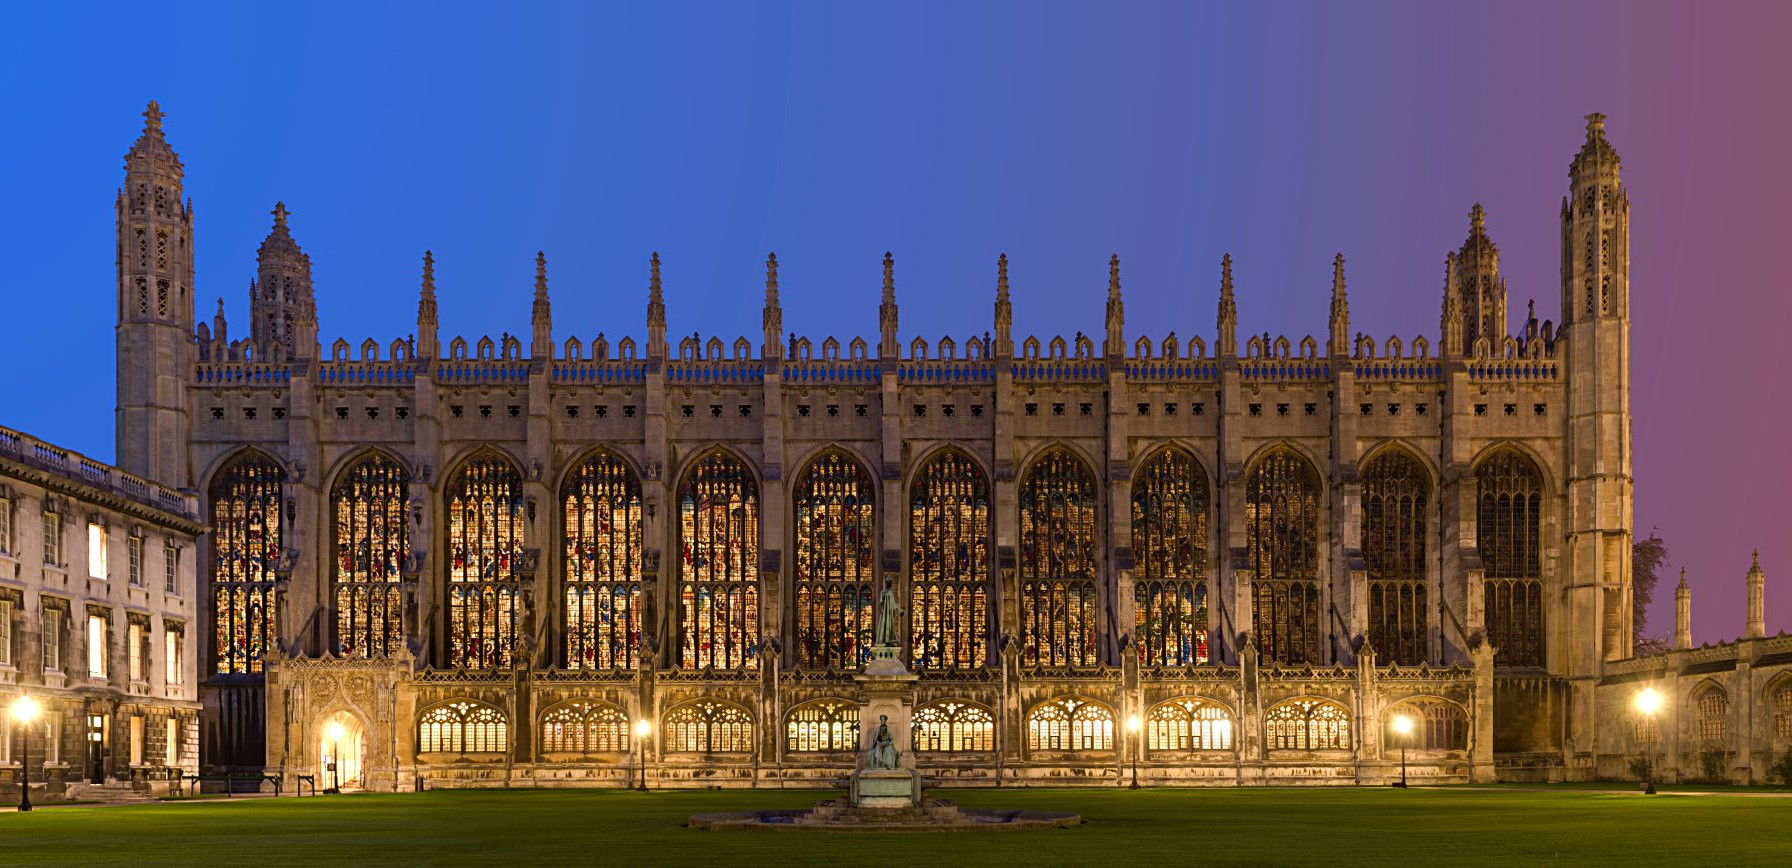
\includegraphics[width=\textwidth]{figs/kings.jpg}
	\end{figure}
\end{frame}


%------------------------------------------------
\begin{frame}
	\frametitle{\faQuestionCircleO~What is the thickness of the ceiling?}
	\begin{figure}[ht]
		\centering
		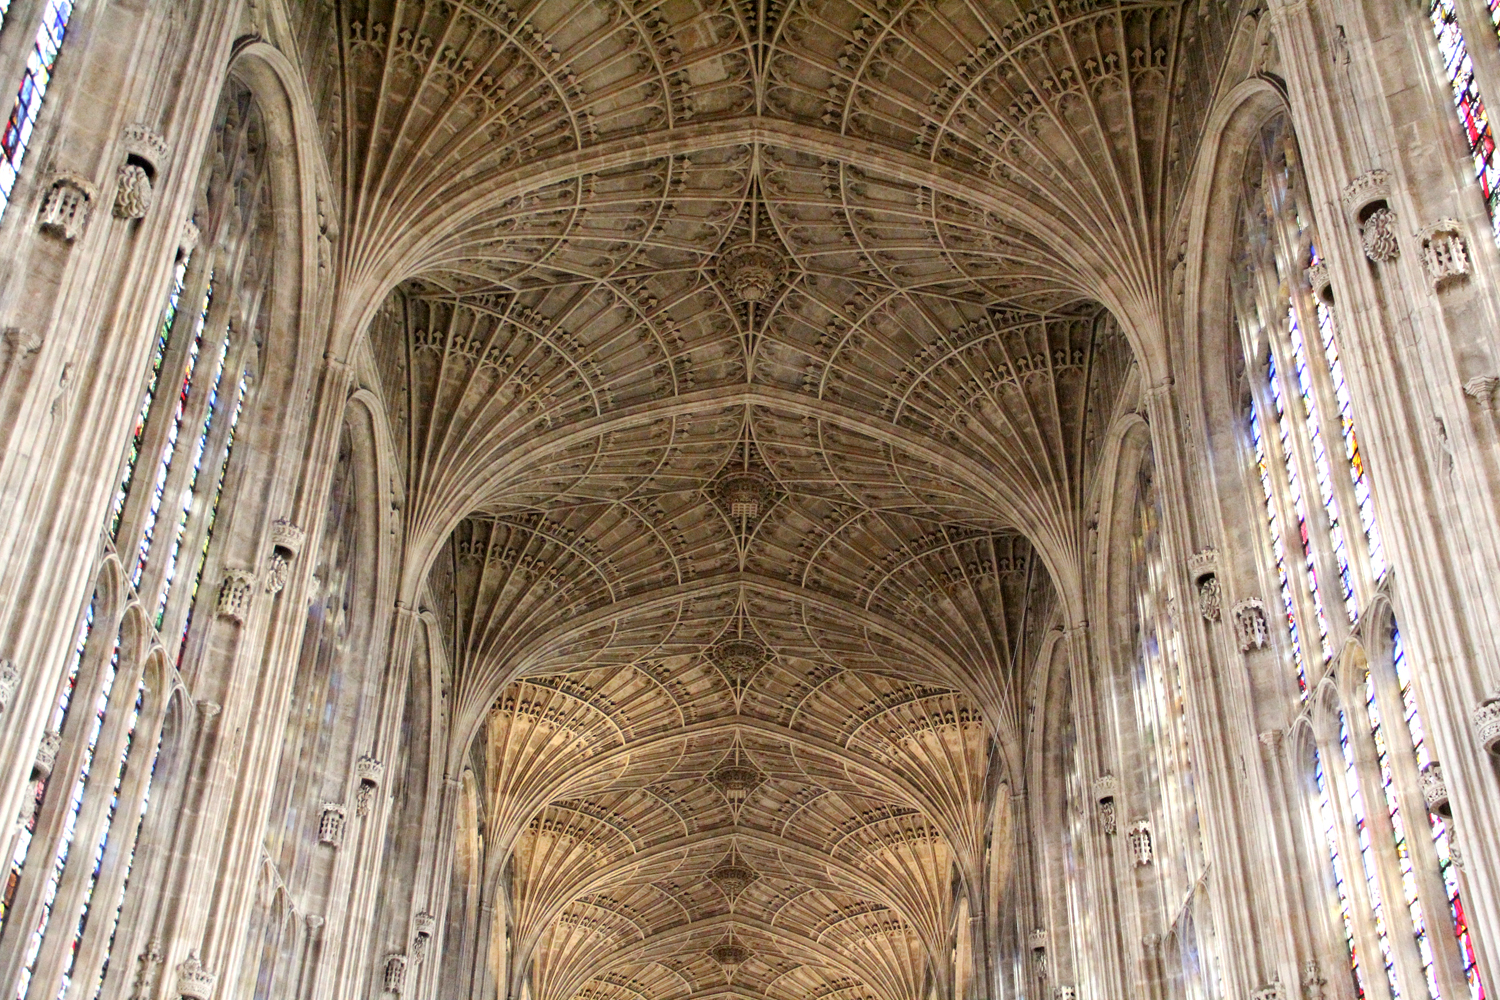
\includegraphics[width=0.8\textwidth]{figs/fanvaults.jpg}
	\end{figure}
\end{frame}

%------------------------------------------------
\begin{frame}
	\frametitle{From arches to fan vaults}
	\begin{figure}[ht]
		\centering
		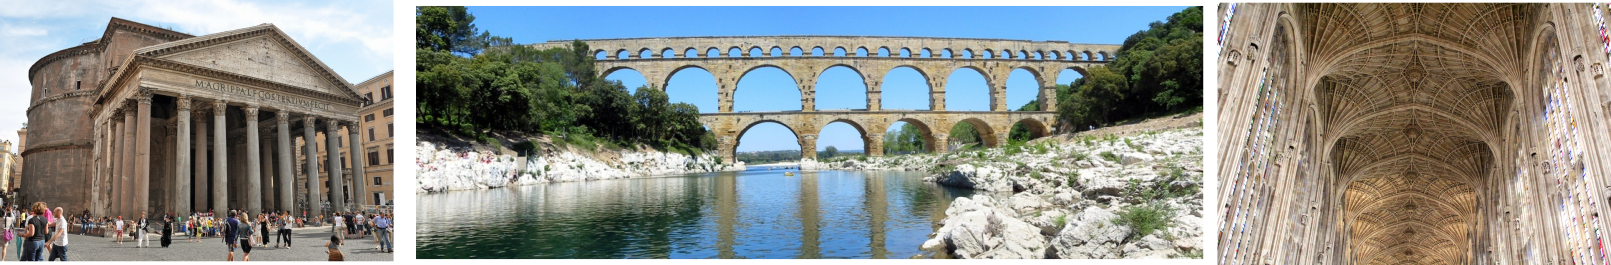
\includegraphics[width=\textwidth]{figs/arches-fan-vaults.png}
	\end{figure}
\end{frame}

%------------------------------------------------
\begin{frame}
	\frametitle{The fan vaults of King's college}
	\begin{figure}[ht]
		\centering
		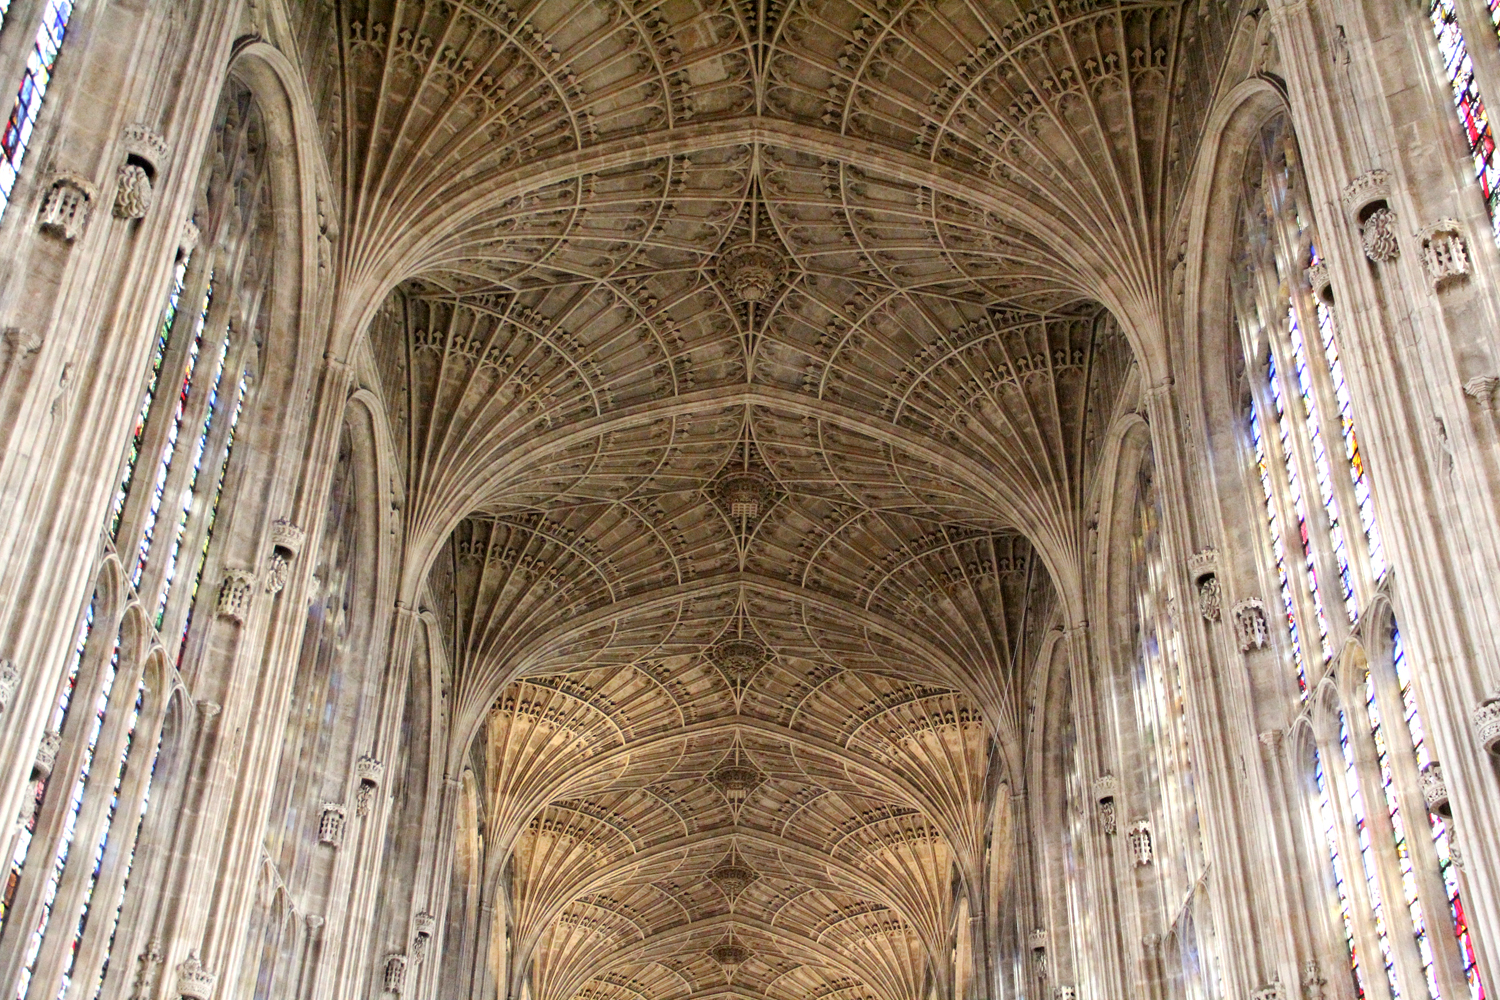
\includegraphics[width=0.8\textwidth]{figs/fanvaults.jpg}
	\end{figure}
\end{frame}

\note{King's college fan vaults were built in 1441}

%------------------------------------------------
\begin{frame}
	\frametitle{Catenary}
	\begin{figure}[ht]
		\centering
		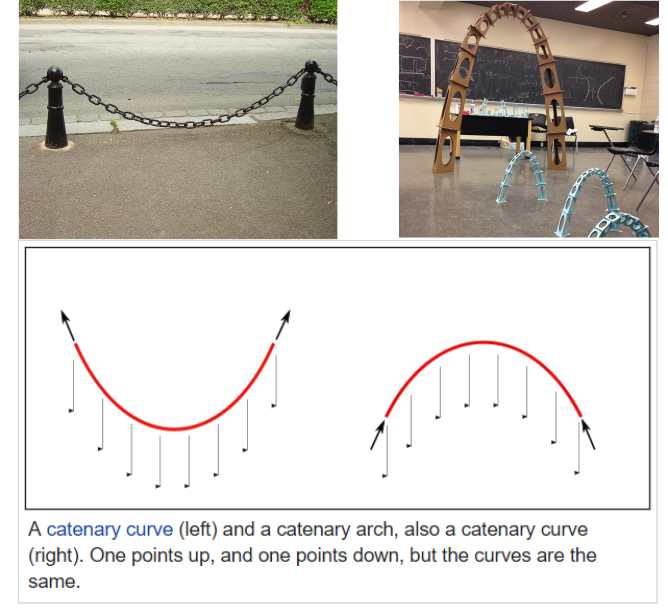
\includegraphics[width=0.65\textwidth]{figs/catenary.png}
	\end{figure}
\end{frame}

\note{The English architect Robert Hooke was the first to study the 
	catenary mathematically and in 1675 published an anagram (in Latin) 
	of : "As hangs the flexible line, so but inverted will stand the 
	rigid arch." The arch above Wembley Stadium has the shape of a 
	catenary and Christopher Wren also intended to use it in St. 
	Paul's dome }

%------------------------------------------------
\begin{frame}
	\frametitle{Catenary, caternary \dots everywhere}
	\begin{figure}[ht]
		\centering
		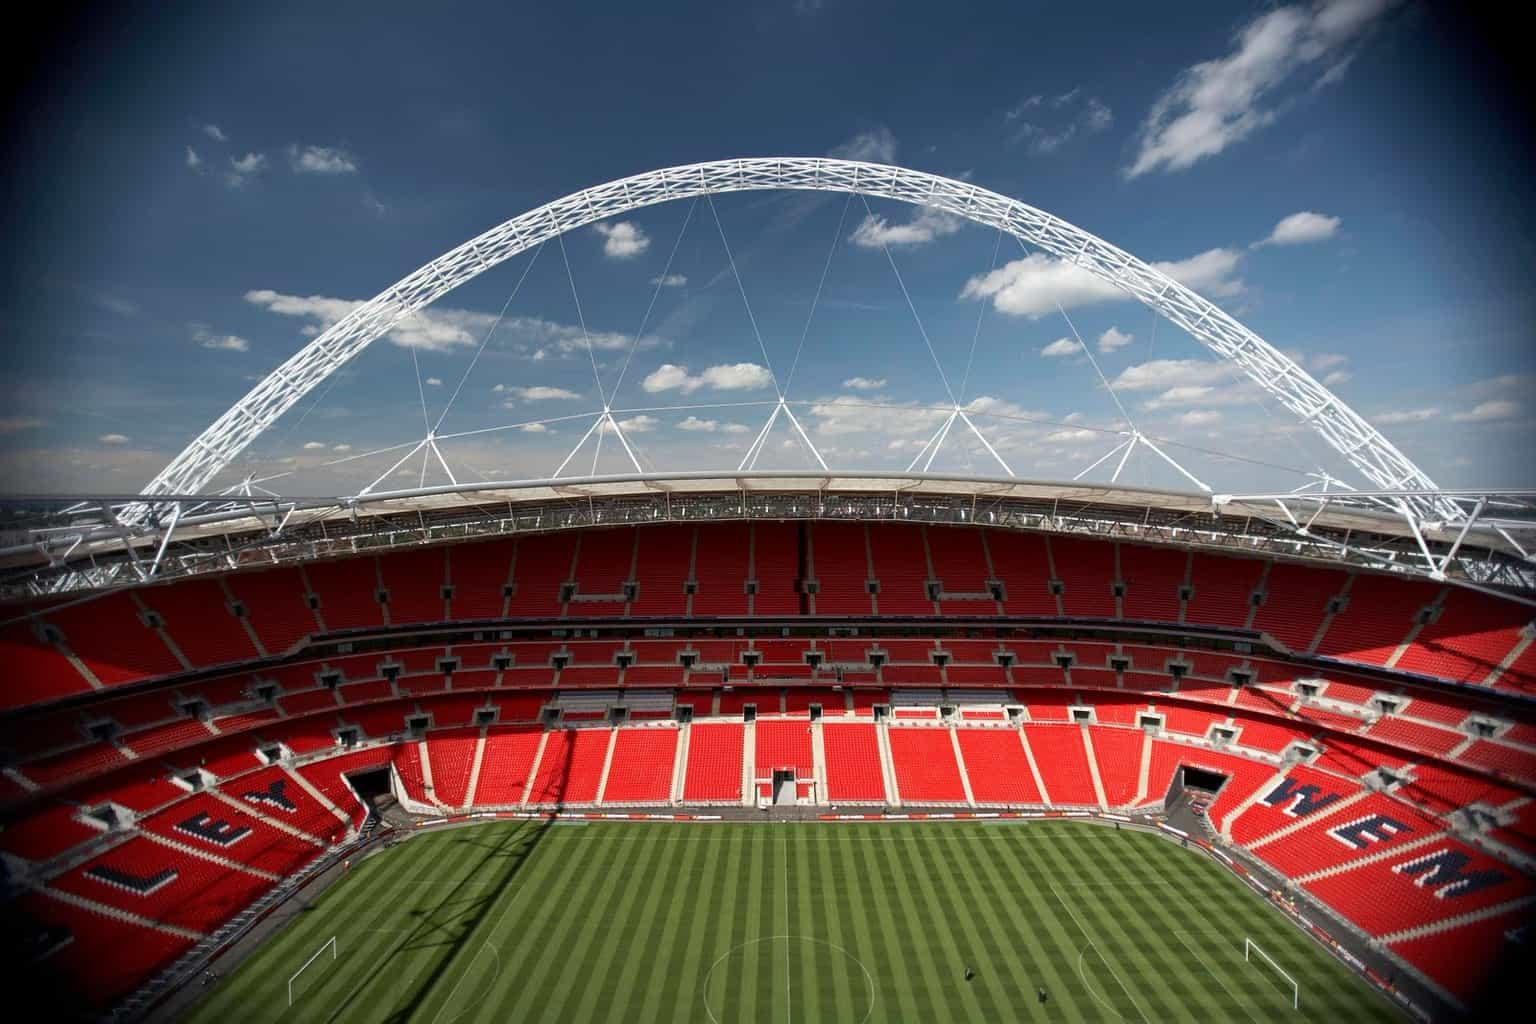
\includegraphics[width=0.95\textwidth]{figs/wembley.jpg}
	\end{figure}
\end{frame}

%------------------------------------------------
\begin{frame}
	\frametitle{Sagrada Familia}
	\begin{figure}[ht]
		\centering
		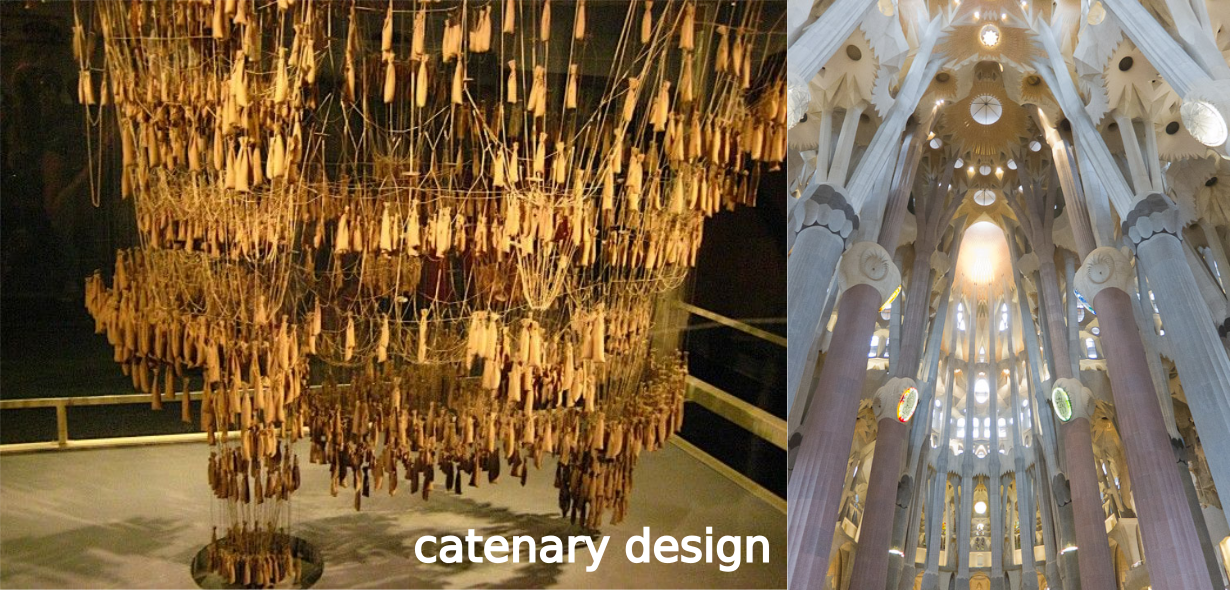
\includegraphics[width=\textwidth]{figs/sagrada-familia.png}
	\end{figure}
\end{frame}

\note{Antoni Gaudi i Cornet (1852-1926) was a well-known architect from Spain.
	Gaudi used catenary arches in many of his projects. One of Gaudi's greatest works however became the Temple of the Holy Family (the Sagrada Familia) in Barcelona.}

%------------------------------------------------
\begin{frame}
	\frametitle{\faQuestionCircleO ~What is this shape?}
	\begin{figure}[ht]
		\centering
		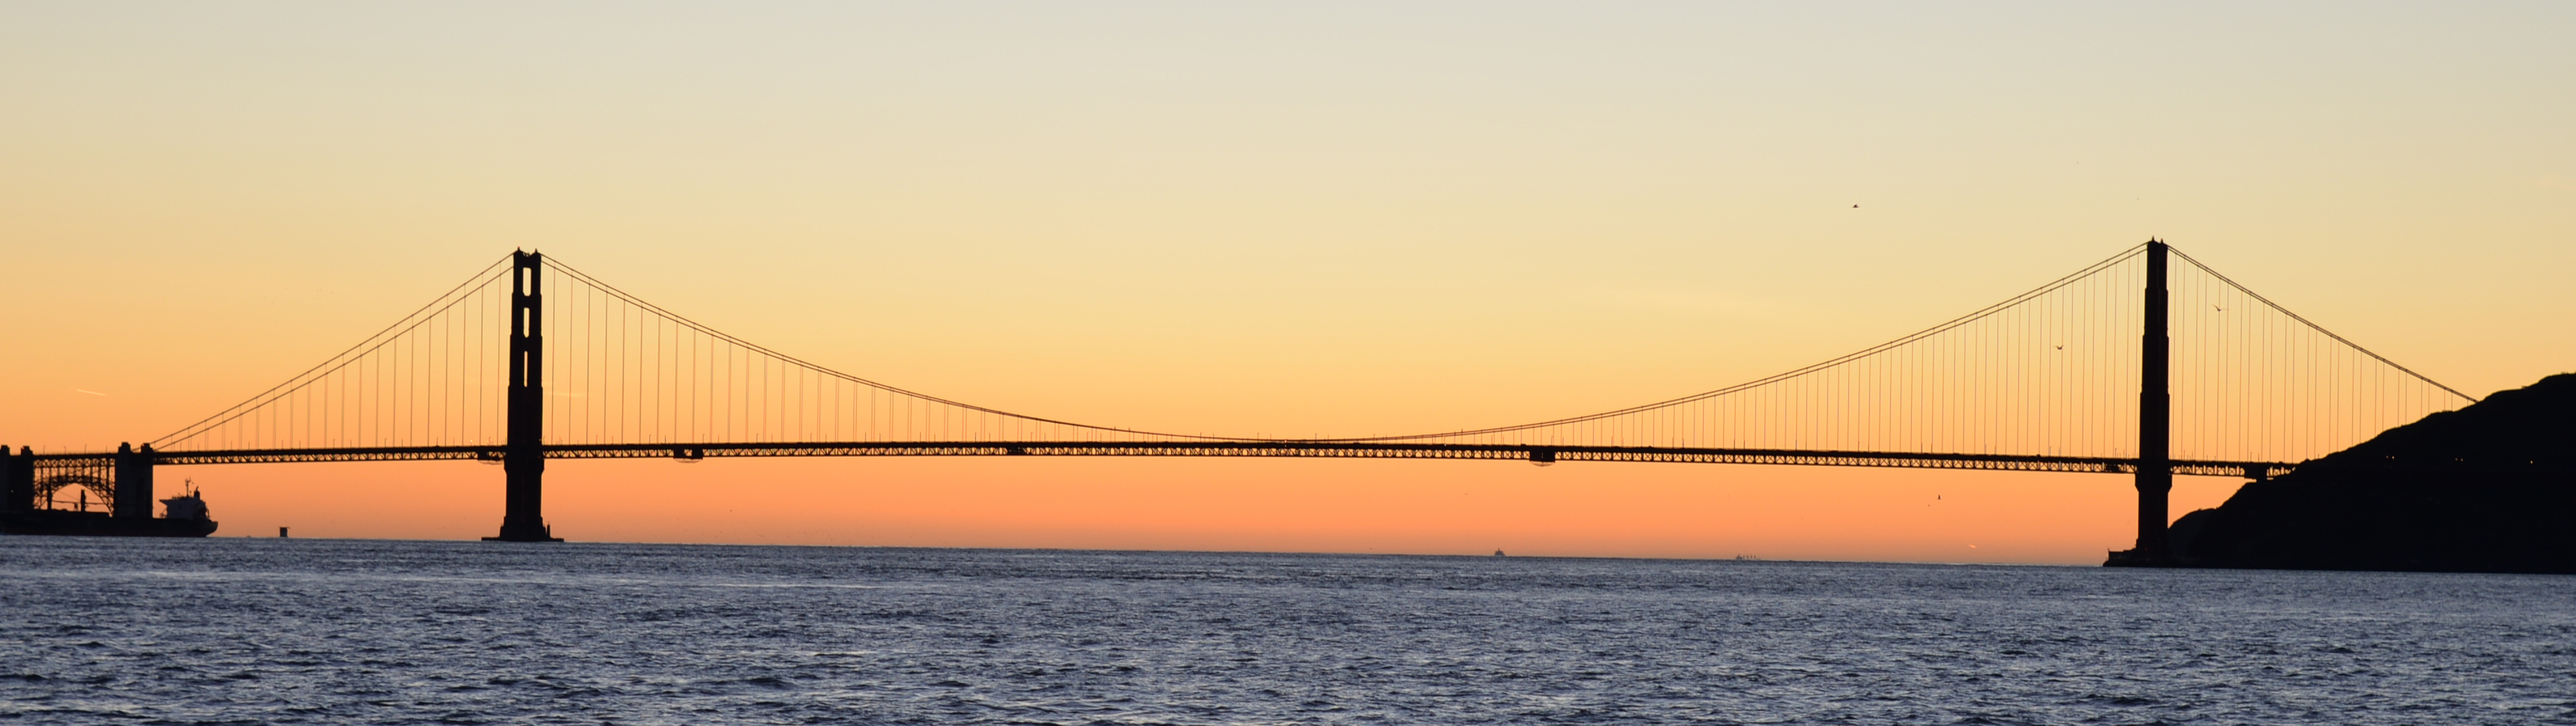
\includegraphics[width=\textwidth]{figs/parabola.jpg}
	\end{figure}
\end{frame}


%------------------------------------------------
\begin{frame}
	\frametitle{Catenary vs Parabola}
	\begin{figure}[ht]
		\centering
		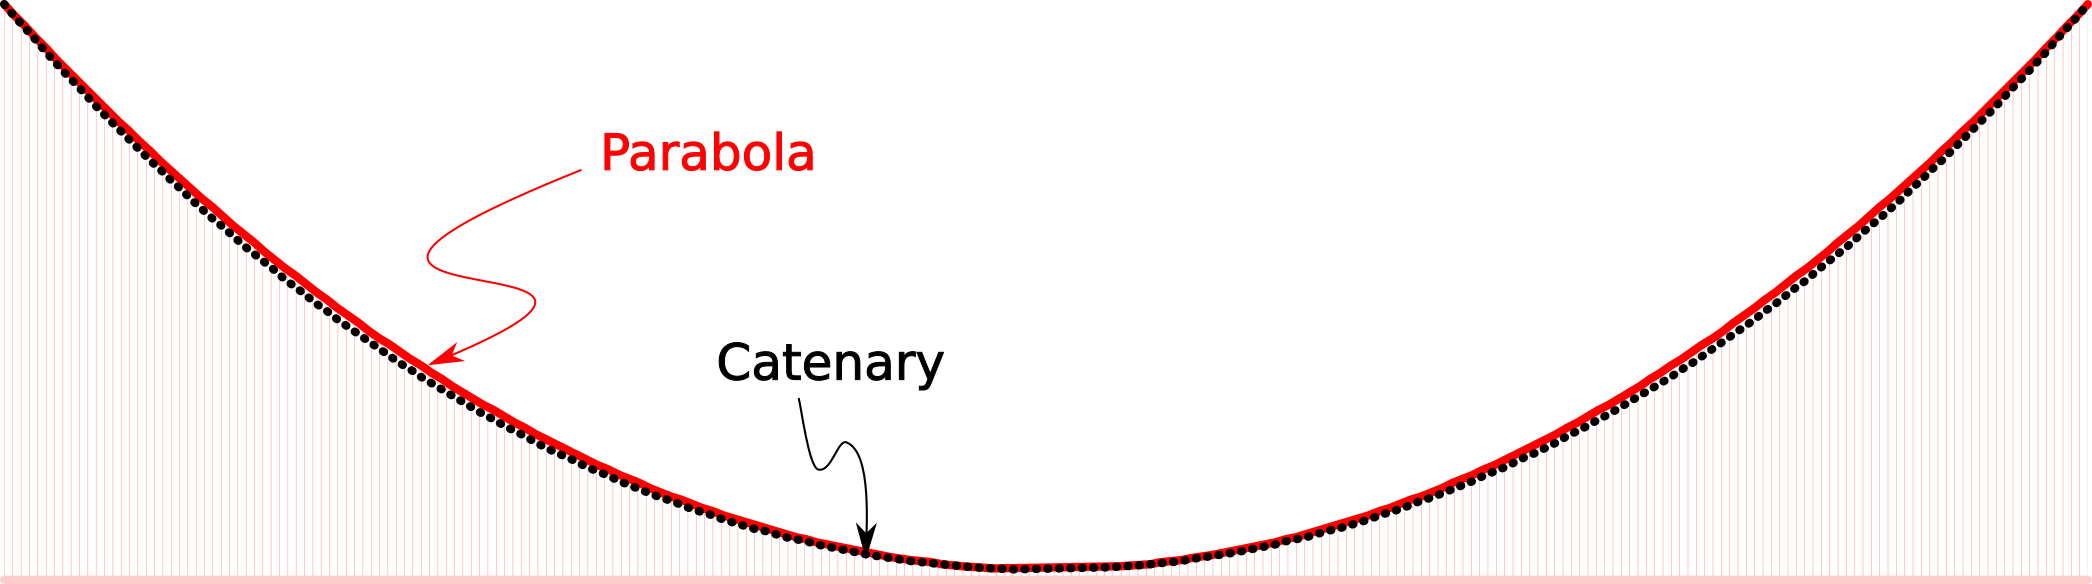
\includegraphics[width=\textwidth]{figs/catenary_parabola.png}
	\end{figure}
\end{frame}
\end{document}
